%\documentclass[preprint,tightenlines,showpacs,showkeys,floatfix,
%nofootinbib,superscriptaddress,fleqn]{revtex4} 
\documentclass[tightenlines,floatfix,nofootinbib,superscriptaddress,fleqn]{revtex4} 
%\documentclass[aps,epsfig,tightlines,fleqn]{revtex4}
\usepackage{kotex}
\usepackage[HWP]{dhucs-interword}
\usepackage[dvips]{color}
\usepackage{graphicx}
\usepackage{bm}
%\usepackage{fancyhdr}
%\usepackage{dcolumn}
\usepackage{defcolor}
\usepackage{amsmath}
\usepackage{amsfonts}
\usepackage{amssymb}
\usepackage{amscd}
\usepackage{amsthm}
\usepackage[utf8]{inputenc}
%\pagestyle{fancy}

\begin{document}

\title{\Large 2022년 2학기 물리학 II}

\author{Hui-Jae Lee} 
\email{hjlee6674@inha.edu}
\affiliation{Hadron Theory Group, Department of Physics,
  Inha  University, Incheon 22212, Republic of Korea }
\date{Autumn Semester, 2022}

\author{김현철\footnote{Office: 5S-436D (면담시간 매주
    수요일-16:15$\sim$19:00)}} 
\email{hchkim@inha.ac.kr}
\affiliation{Hadron Theory Group, Department of Physics,
  Inha  University, Incheon 22212, Republic of Korea }
\date{Autumn Semester, 2022}

\maketitle



\section*{\large Quiz 11}
\noindent {\bf 문제 1 [20pt].} 
최대전압이 220 V인 교류전원에 10.0 $\mathrm{\Omega}$의 저항을 연결하였을 때,
저항에 흐르는 유효전류와 평균 소비전력을 구하여라.

\noindent {\bf 풀이 : } 
교류전원의 최대 전압을 $\mathcal{E}_0$라고 하면 저항에 걸리는 유효전압 $\mathcal{E}_{rms}$와
저항에 흐르는 유효전류 $I_{rms}$는 다음의 관계에 있다.
\begin{align}
  \mathcal{E}_{rms} = \frac{\mathcal{E}_0}{\sqrt{2}},\,\,\,
  \mathcal{E}_{rms} = I_{rms}R.
\end{align}
$R$은 저항의 저항값이다. 또한 평균 소비전력 $\left<P\right>$는
\begin{align}
  \left<P\right> = I_{rms}^2R
\end{align}
이다. 따라서 유효전류 $I_{rms}$는
\begin{align}
  I_{rms} = \frac{\mathcal{E}_0}{\sqrt{2}R}=
  \frac{220~\mathrm{V}}{\sqrt{2}\times 10.0~\mathrm{\Omega}} = 15.6~\mathrm{A}
\end{align}
이고 평균 소비전력  $\left<P\right>$는
\begin{align}
  \left<P\right> = \frac{\mathcal{E}^2_0}{\sqrt{2}R}
  =\frac{(220~\mathrm{V})^2}{\sqrt{2}\times 10.0~\mathrm{\Omega}}
  =3420~\mathrm{W}
\end{align}
이다.
\vspace{1cm}

\noindent {\bf 문제 2 [20pt].}
어떤 축전기의 양단에 진동수가 60.0 Hz이고 240.0 V의 최대 전압진폭을
가지는 전원이 연결되어 축전기에 1.20 A의 전류가 흐른다. 전기용량은 얼마인가?

\noindent {\bf 풀이 : } 
전원의 진동수와 최대 전압을 $\omega$, $\mathcal{E}_0$, 축전기에 흐르는 전류를 
$I$, 축전기의 전기용량을 $C$라 하자. 전원에 의한 교류 전압 $\mathcal{E}(t)$는
시간에 대한 함수로 표현이 가능하다.
\begin{align}
  \mathcal{E}(t) = \mathcal{E}_0\sin\omega t.
\end{align} 
또한 축전기에 쌓이는 전하량을 $Q(t)$라 하면 전원에 의한 전압 $\mathcal{E}(t)$에
의해
\begin{align}
  \mathcal{E}(t) - \frac{Q(t)}{C} = 0 
\end{align}
이 성립한다. 따라서 $Q(t)$는
\begin{align}
  Q(t) = C\mathcal{E}(t) = C\mathcal{E}_0\sin\omega t
\end{align}
이고 전류 $I(t)$는 전하 $Q(t)$의 시간 당 변화량이므로
\begin{align}\label{eq:2-1}
  I(t) = \frac{dQ(t)}{dt} = C\omega\mathcal{E}_0\cos\omega t = I_0\cos\omega t
\end{align}
로 쓸 수 있다. $I_0$는 최대 전류이다. 축전기에 흐르는 유효 전류 $I_{rms}$의 크기가
1.20 A이므로
\begin{align}
  I_{rms} = \frac{I_0}{\sqrt{2}}=\frac{C\omega \mathcal{E}_0}{\sqrt{2}}
\end{align}
이고 따라서 전기용량 $C$는
\begin{align}
  C = \frac{\sqrt{2}I_{rms}}{\omega \mathcal{E}_0}
  =\frac{\sqrt{2}(1.20~\mathrm{A})}{(60.0~\mathrm{Hz})(240.0~\mathrm{V})}
  =1.18\times 10^{-4}~\mathrm{F}
\end{align}
이다.
\vspace{1cm}

\noindent {\bf 문제 3 [50pt].}
그림~\ref{fig:3}과 같이 저항과 인덕터가 병렬로 연결되어 있고, 여기에
교류전압 $\mathcal{E}=\mathcal{E}_{\mathrm{max}}\cos\omega t$가 걸려
있다. 
\begin{figure}[htp]
  \centering
  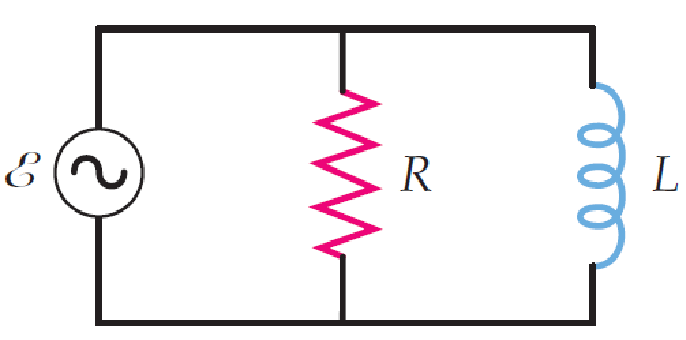
\includegraphics[scale=0.4]{qfig11-20221024-1.pdf}
  \caption{\textbf{문제 3}}
  \label{fig:3}
\end{figure}
\begin{itemize}
\item[(가)] 저항에 흐르는 전류가 
$I_R=(\mathcal{E}_{\mathrm{peak}}/R)\cos\omega t$와 같이 주어짐을
보여라. 여기서 $\mathcal{E}_{\mathrm{peak}}$은 주기함수가 최대가 되는
지점에서 $\mathcal{E}(t)$ 값이다. 
\item[(나)] 인덕터에 흐르는 전류는
  $I_L=(\mathcal{E}_{\mathrm{peak}}/X_L)\cos(\omega t -90^\circ)$임을
  보여라. 
\item[(다)] 교류 전압의 기전력이 걸려 있는 데서 
  $I=I_R+I_L=I_{\mathrm{peak}} \cos(\omega t-\delta)$의 전류가 흐름을
  보여라. 여기서
  $I_{\mathrm{peak}}=(\mathcal{E}_{\mathrm{peak}}/Z)$이다. 
\end{itemize}

\noindent {\bf 풀이 : } 
\begin{itemize}
  \item[(가)]
  저항과 코일이 병렬로 연결되어 있으므로 저항과 코일에 걸리는 전압은 교류전압
  $\mathcal{E}$와 같다. 따라서 저항에 흐르는 전류 $I_R$은
  \begin{align}
    I_R = \frac{\mathcal{E}}{R} = \frac{\mathcal{E}_\mathrm{{max}}}{R}\cos\omega t
  \end{align}
  이고 주기함수가 최대가 되는 지점에서 $\mathcal{E}(t)$는 $\mathcal{E}_\mathrm{{max}}$이므로
  \begin{align}\label{eq:3-1}
    I_R =\frac{\mathcal{E_\mathrm{{max}}}}{R}\cos\omega t
    =\frac{\mathcal{E}_\mathrm{{peak}}}{R}\cos\omega t
  \end{align}
  로 쓸 수 있다.
  \item[(나)]
  인덕터에 흐르는 전류 $I_L$을 구하기 위해 우선 인덕터에 걸리는 전압 
  $\mathcal{E}_L$을 구하자. (가)에서 말한 바와 같이 $\mathcal{E}_L$은
  교류전압 $\mathcal{E}$와 같으므로
  \begin{align}
    \mathcal{E}_L = \mathcal{E}_{\mathrm{max}}\cos\omega t
  \end{align}
  인덕터 회로의 경우
  \begin{align}
    \mathcal{E}_L - L\frac{dI_L}{dt} = 0
  \end{align}
 이다. $L$은 인덕턴스이다. 따라서 $I_L$은 
 \begin{align}
  I_L = \frac{\mathcal{E_\mathrm{{max}}}}{L} \int^t_0 \cos \omega t'\,dt'
  =\frac{\mathcal{E_\mathrm{{max}}}}{\omega L} \sin \omega t
  \end{align}
  이고 $X_L = \omega L$, $\sin \omega t = \cos (\omega t-90^\circ)$ 이므로
  \begin{align}\label{eq:3-2}
    I_L = \frac{\mathcal{E_\mathrm{{peak}}}}{X_L} \cos (\omega t-90^\circ)
  \end{align}
  와 같다.
  \item[(다)]
  식~\eqref{eq:3-1}, \eqref{eq:3-2}로부터 $I= I_R+I_L$은
  \begin{align}
    I = I_R+I_L = \frac{\mathcal{E}_\mathrm{{peak}}}{R}\cos\omega t
    +\frac{\mathcal{E_\mathrm{{peak}}}}{X_L} \sin \omega t
  \end{align}
  인데 $A\cos x+B\sin x$꼴은 다음과 같이 계산할 수 있다.
  \begin{align}
    \begin{split}
      A\cos x+B\sin x &= \sqrt{A^2+B^2}\left(\frac{A}{\sqrt{A^2+B^2}}\cos x
      +\frac{B}{\sqrt{A^2+B^2}}\sin x\right)  \\
      &=\sqrt{A^2+B^2}(\cos \delta\cos x+\sin \delta\sin x) \\
      &=\sqrt{A^2+B^2}\cos(x-\delta).
    \end{split}
  \end{align}
  $A = \mathcal{E_\mathrm{{peak}}}/R$, $B = \mathcal{E_\mathrm{{peak}}}/X_L$이고
  $x = \omega t$라 하면
  \begin{align}
    \begin{split}
      I &= \sqrt{\left(\frac{\mathcal{E_\mathrm{{peak}}}}{R}\right)^2
      +\left(\frac{\mathcal{E_\mathrm{{peak}}}}{X_L}\right)^2}
      \cos(\omega t-\delta) \\
      &= \mathcal{E_\mathrm{{peak}}}\sqrt{\frac{1}{R^2}+\frac{1}{X_L^2}}
      \cos(\omega t-\delta)
    \end{split}
  \end{align}
  으로 쓸 수 있다. 저항과 코일이 병렬로 연결되어 있으므로 임피던스 $Z$는
  \begin{align}
    \frac{1}{Z} = \sqrt{\left(\frac{1}{R}\right)^2+\left(\frac{1}{X_L}\right)^2}
  \end{align}
  로 정의되므로 전류 $I$는
  \begin{align}
    I = \frac{\mathcal{E_\mathrm{{peak}}}}{Z}\cos(\omega t-\delta)
  \end{align}
  와 같다.
\end{itemize}

\vspace{1cm}

\noindent {\bf 문제 4 [50pt].}
$RLC$ 직렬회로에 교류전원을 연결하고 출력 전압은 $R$과 $L$을 연결한 조합의
양단에서 얻는다. 출력 전압과 입력전압의 비를 각진동수 $\omega$의
함수로 구하라. 매우 높은 진동수에서는 이 값이 1에 가까워 짐을 보여라. 

\noindent {\bf 풀이 : } 
입력전압을 $\mathcal{E}$, 저항, 코일, 축전기에 가해지는 전압을 $\mathcal{E}_R$,
$\mathcal{E}_L$, $\mathcal{E}_C$라고 하면
\begin{align}\label{eq:4-1}
  \mathcal{E} - \mathcal{E}_R - \mathcal{E}_L - \mathcal{E}_C
  =\mathcal{E} - IR - L\frac{d I}{dt} -\frac{Q}{C}  =0
\end{align}
를 만족한다. $R$, $L$, $C$는 각각 저항, 리액턴스, 전기용량이다. 입력전압을
\begin{align}
  \mathcal{E}(t) = \mathcal{E}_0\cos\omega t
\end{align}
라고 가정하자. 저항, 코일, 축전기가 모두 연결되어 있으므로 회로에 흐르는 전류 $I(t)$에
$\phi$만큼의 위상차가 존재한다고 하면
\begin{align}
  I(t) = \frac{\mathcal{E}_0}{Z}\cos(\omega t-\phi),\,\,\,
  Z = \sqrt{R^2+\left(\omega L-\frac{1}{\omega C}\right)^2}
\end{align}
로 쓸 수 있다. $Z$는 회로의 임피던스이다. 저항에서 전압강하의 위상은 $I(t)$와 같으므로
\begin{align}
  \mathcal{E}_R = IR = \frac{\mathcal{E}_0 R}{Z}\cos(\omega t-\phi)
\end{align}
이고 코일에서 전압강하의 위상은 $\pi/2$만큼 빠르다. 반면에 축전기에서의 위상은 
$\pi/2$만큼 느리므로 식~\eqref{eq:4-1}로 부터
$\mathcal{E}_L$, $\mathcal{E}_C$는
\begin{align}
  \mathcal{E}_L = \frac{\mathcal{E}_0\omega L}{Z}\sin(\omega t-\phi) ,\,\,\,
  \mathcal{E}_C = -\frac{\mathcal{E}_0}{Z\omega C}\sin(\omega t-\phi) 
\end{align}
와 같다. 출력전압 $\mathcal{E}_{out}$은 저항과 코일을 연결한 조합의 양단에서 얻으므로
\begin{align}
  \mathcal{E}_{out} = \mathcal{E}_R+\mathcal{E}_L
  =\mathcal{E}-\mathcal{E}_C
\end{align}
이다. 따라서 입력전압 $\mathcal{E}$와 출력전압 $\mathcal{E}_{out}$의 비는
\begin{align}\label{eq:4-2}
  \frac{\mathcal{E}_{out}}{\mathcal{E}}
  =\frac{\mathcal{E}-\mathcal{E}_C}{\mathcal{E}}
  =1+\frac{\sin(\omega t-\phi)}{Z\omega C\cos\omega t}
\end{align}
로 표현할 수 있다. 이제 $\omega$가 매우 크다고 가정하자. 식~\eqref{eq:4-2}의 마지막 항은
\begin{align}
  \frac{\sin(\omega t-\phi)}{Z\omega C\cos\omega t}
  =\frac{1}{C}\frac{\sin(\omega t-\phi)}{\sqrt{\omega^2R^2
  +\left(\omega^2 L-\frac{1}{C}\right)^2}\cos\omega t}
\end{align}
로 쓸 수 있는데 $\omega$가 매우 크므로
\begin{align}
  \frac{1}{Z}=\frac{1}{\sqrt{\omega^2R^2
  +\left(\omega^2 L-\frac{1}{C}\right)^2}}
  \longrightarrow 0
\end{align}
이고 위상차  $\phi$는
\begin{align}
  \tan \phi = \frac{\omega L - \frac{1}{\omega C}}{R}
  \longrightarrow \infty
\end{align}
$\omega$가 커짐에 따라 같이 커진다. 따라서 $\phi = \pi/2$로 볼 수 있고
\begin{align}
  \frac{\sin(\omega t-\phi)}{\cos\omega t}=1
\end{align} 
이 된다. 최종적으로 $\omega$가 매우 클 때 입력전압과 출력전압의 비는 
\begin{align}
  \frac{\mathcal{E}_{out}}{\mathcal{E}}=1+\frac{1}{C}\frac{1}{Z}
  \frac{\sin(\omega t-\phi)}{\cos\omega t}=1
\end{align}
1이 된다는 사실을 확인할 수 있다.
\end{document}

